\chapter{\label{ch:4-gemini}Attosecond electron bunches and X-ray pulses on GEMINI PW} 

\minitoc

\section{Overview}
We successfully measured the intensity of the attosecond duration X-ray harmonics on the ORION SP1 and SP2 beamlines. However, the uncertainties remained large, the geometry sub-optimal and the pulse train exceedingly far from an isolated attosecond pulse. Indeed none of the proposed mechanisms for isolation (polarisation gating, lighthouse technique, etc.) could have any hope of success. The high shot rate, few femtosecond, highly customisable GEMINI PW facility at CLF can address all these points while also providing conditions suitable for the production of attosecond ZVP electron bunches, of course attended by its own suite of technical challenges. The work of the prior chapters of this thesis formed the body of a successful proposal for five weeks of beam time at the facility with shot dates planned for Summer 2024. This chapter outlines the extensive planning process initiated over a year before the experiment itself.

There are three primary experimental goals. First, to repeat the ORION experiment on GEMINI PW with optimised geometry and thus resolve and measure the absolute intensity of X-ray harmonics, detailed in Section X. Second, to simultaneously observe ZVP electron bunches in transmission and the HHG signal they generate in reflection, detailed in Section X. Finally, to apply the X-ray harmonic beam in a proof of principle Laue diffraction setting described in Section X. Section X addresses the subject of laser contrast, a much thornier issue for the few femtosecond GEMINI beamline compared to ORION and covers the parallel experiment proposed by collaborators at Queen's University Belfast to provide some illumination to the problem at hand. Note that no petawatt class few femtosecond laser facility has observed harmonics at oblique incidence. This section will also detail the strategy of contingency should the contrast prove to be too poor for the production of harmonics. Not discussed in this chapter is the work undertaken by Elliot Denis to perform spectro-spatial encoding and thus temporally resolve chirped HHG.

% TODO get the name of what Ellit it doing.

% TODO replace HHG with SHHG

CAD drawings overview where to put you?

The experimental geometry is relatively simple. Post \ac{DPM} contrast enhancement, the GEMINI PW South (S) beam is focused by an $f/2$ parabola onto the solid density target at \qty{45}{\degree} \ac{AOI} and p-polarisation, directing the specularly reflected X-ray beam to the West side of the chamber. XUV and X-ray spectrometers aligned to the target in the specular direction will observe the reflected harmonic beam.

\section{X-ray harmonics on GEMINI PW}
Naturally, the first action is to repeat the ORION experiment at GEMINI PW. For this purpose, the Oxford Engineering Department is designing and building a replica OHREX spectrometer to perform the measurement with OHREX crystals borrowed from AWE. The lower energy KAP (100) OHREX crystal listed in Table \ref{tab:dispersion} is more suited to GEMINI PW due to the lower energy of the beamline compared to ORION. Regardless, the quartz crystals will also be fielded. 

A 1D PIC simulation of the GEMINI PW beamline for the planned geometry predicts harmonics will be resolved for the KAP energy range.
[INSERT PIC SIMS HERE].


The technical complexity of the OHREX spectrometer is entirely attached to the spherically bent OHREX crystals, thus reducing the challenges of alignment \cite{beiersdorferLineshapeSpectroscopyVery2016}. It is designed to be relatively insensitive to the distances between source and crystal (2.4 m) and from crystal to image plane (0.524 m). Indeed, previous experiments deemed it unnecessary to adjust the OHREX bellows to access the best focus. Variation in the angle of incidence from \qty{38.7}{\degree} shifts the spectral image away from the nominal energy range. 
% TODO am I doing this? The variation is relatively sensitive, for the quartz ($10\bar{1}1$) crystal, a change in energy of \qty{8}{\%} is obtained by a change in angle of \qty{50}{\mu rad} \cite{macdonaldAbsoluteThroughputCalibration2021}. Nevertheless, t
The alignment of the crystal planes to the crystal surface enables the relative convenience of optical alignment. Initial shots will use IP to check for any light leakage and to confirm alignment. Switching to the Raptor Photonics Eagle XV in vacuum X-ray CCD camera (EA4240XV-BN-CL) \cite{EagleXVVacuum} to utilise the high shot rate on GEMINI PW. The CCD camera must be liquid cooled, thus for the prevention of damaging condensation forming on the camera window a manual gate valve is required to isolate the OHREX when pumping the main chamber (waiting for the camera to reach acceptable temperatures while under vacuum would be prohibitively long). With $2048 \times 2048$ active pixels of size \qty{13.5}{\mu m} $\times$ \qty{13.5}{\mu m}, not all of the 4 cm crystal image can be captured by the camera.


A parameter scan of \ac{XHHG} as a function of $S$ can be performed by varying the laser intensity, via beam apodisation, and the target material. The majority of shots will use target wheels of the relatively high damage threshold fused silica with the plan to advance to a kapton tape. The fused silica targets are chemically etched in one corner to aide alignment.
% TODO cite the below
Since HHG is suppressed for circularly polarised light, bremmstrahlung emission and/or other X-ray production mechanisms can somewhat be ruled out by comparing the \ac{XHHG} signal observed for p- and circularly- polarised light, produced via a quarter wave plate. However, this is not fully the case at \qty{45}{\degree} \ac{AOI} and plasma heating is reduced, reducing the temperature of the emitting plasma.

Filtering is necessary to reject the high intensity low order harmonics, however, for photon energies in the 600 eV range, the standard beryllium filter transmission is too low. Instead 400 nm of aluminium flash-coated onto 1 micron of mylar will be used for the KAP crystal, corresponding to a transmission of \qty{16}{\%} at 600 eV.

It is essential to check there is suitable resolution in both the spectrometer and the CCD camera for harmonic observation. For the highest energy crystal, nominal photon energy of 2.405 keV, 96 harmonics sit in the range accessed by the crystal, corresponding to a fractional energy $\Delta E/E =$ \num{6.45e-4} between harmonics. At  $\Delta E/E =$ \num{1e-4}, the OHREX crystal resolution is sufficient, however it may not resolve the harmonics' spectral shape. Those 96 harmonics are spread over the 4 cm crystal image. At a resolution of \qty{13.5}{\mu m}, the CCD camera has 31 pixels between harmonics and the harmonic width is about a pixel.

% TODO KAPTON sims
sims:
Running new SiO2 HHG sim, hopefully this will show that we have a better efficiency than the previous simulation. Then pop that in here.

A previous experiment measured the GEMINI DPM setup produced a reduction in peak pulse intensity of \qty{50}{\%}. Applying ROM and hole boring theory to a fused silica target and accounting for filtering and assuming no merging of harmonics, one can anticipate signals at the OHREX crystal position of \qty{19.6}{\mu J.sr^{-1}} per harmonic at 0.6 keV for the KAP crystal and \qty{1.89}{\mu J.sr^{-1}} per harmonic at 2.405 keV for the quartz ($10\bar{1}1$) crystal. Orienting the OHREX for s-polarisation to maximise the signal at the image plane, this corresponds to an average of 3.4 photons per pixel and 0.20 photons per pixel respectively. The quantum efficiency of the detector is close to \qty{100}{\%}. These numbers are no smaller than the ORION experiment while the background will be lower due to the order of magnitude lower energy on target. Thus, there should be adequate statistics to observe these signals.

\section{First observation of ZVP electron bunches}
The second phase of the GEMINI PW experiment is to observe ZVP electron bunches (both mass-limited and bulk) for the first time. There has been some experimental evidence of attosecond and nano-Coulomb electron bunch generation from nano-targets \cite{cardenasSubcycleDynamicsRelativistic2019,hornyGenerationSingleAttosecond2021} and in reflection from solids \cite{linIsolatedAttosecondElectron2020, thevenetVacuumLaserAcceleration2016} with the latter demonstrating satisfaction of the precise conditions for \ac{VLA} to 10 MeV for a mildly relativistic laser pulse ($a_0 \approx 3.1$). These experiments have guided the planning process for this experiment stage.

This experiment aspires to produce mass-limited ZVP electron bunches in the configuration simulated in Figure \ref{fig:experimentsetuphhgbunches2}. % TODO repeat this simulation with Silicon wafer target
\begin{figure}
	\centering
	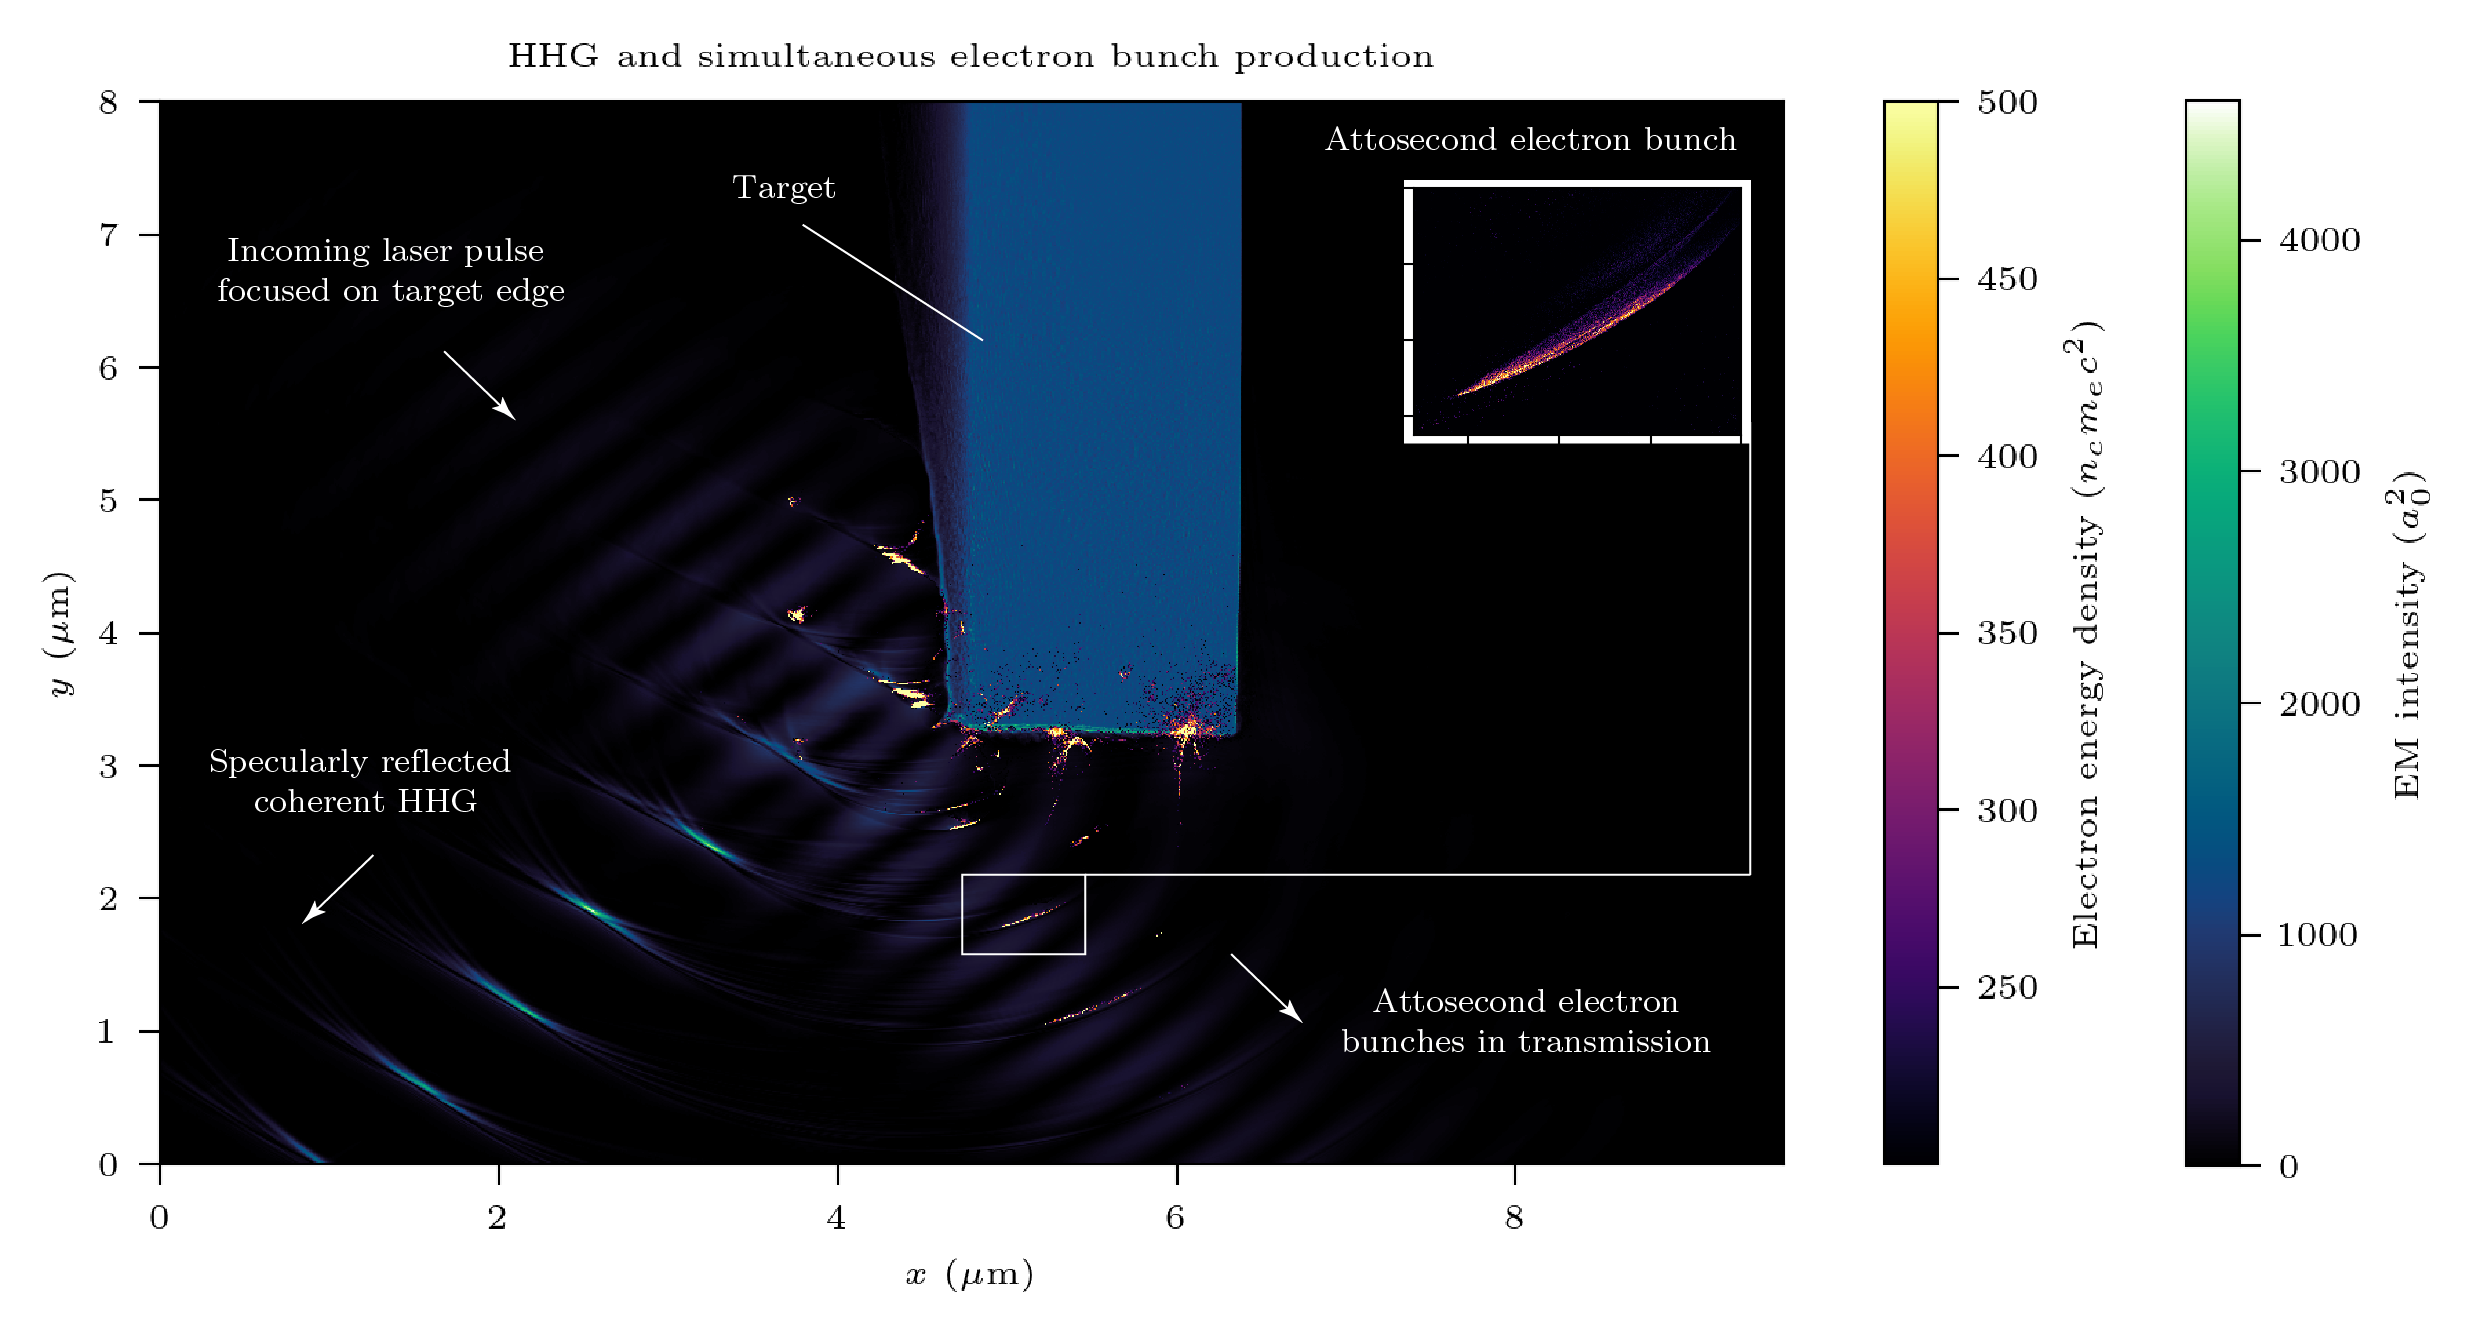
\includegraphics[width=1\linewidth]{figures/zvp/Experiment_setup_HHG_bunches2}
	\caption[Planned GEMINI-PW experimental setup for the measurement of ZVP electron bunches.]{A simulation of the planned GEMINI-PW experimental setup for the measurement of ZVP electron bunches. This novel setup enables the simultaneous measurement of attosecond ZVP electron bunches and their coherent emission of X-ray light. The GEMINI-PW laser pulse is incident at \qty{45}{\degree} on the low density polyethylene target with a preplasma scale length of $0.2\lambda_\mathrm{L}$. For this angle of incidence, transmitted bunches and specularly reflected X-ray harmonics are produced at a frequency of $\omega_\mathrm{L}$.}
	\label{fig:experimentsetuphhgbunches2}
\end{figure}
By focusing the laser pulse onto the edge of a transversely mass-limited target, the emitted electron bunch energies will be maximised. Simulations suggest it should be possible to simultaneously measure the specularly reflected \ac{HHG} and the attosecond electron bunches that produce it. Note via equations \ref{eq:zvp_N} and \ref{eq:zvp_T}, the low density target of Figure \ref{fig:experimentsetuphhgbunches2} will produce larger and more energetic bunches. They are therefore a more practical choice for the experiment relative to the aluminium targets of predominant use in Chapter \ref{ch:2-zvp}. Both bulk and mass-limited ZVP electron bunches will be generated but should be spatially separated at the observation point via conservation of transverse momentum with bulk bunches experiencing no further acceleration phases post ZVP.

It is necessary to conduct PIC code parameter scans for this new geometry. While normal incidence was most convenient for the initial ZVP simulations, oblique incidence is more optimal for \ac{HHG} \cite{gonoskovUltrarelativisticNanoplasmonicsRoute2011, edwardsXRayEmissionEffectiveness2020} and as can be understood from equations \ref{eq:zvp_Tzvp_theta} and \ref{eq:zvp_Uzvp_theta}, the new energy scaling expressions, for the ZVP mechanism. Not only is oblique preferable but it is essential to mitigate damage to the laser optics via back-reflection. The \ac{HHG} beam intensity at focus can be over 1000 times that of the incident laser pulse \cite{quereReflectingPetawattLasers2021}. It is indispensable, therefore, to test the new predictions for oblique incidence energy scalings and total electron bunch charge along with the angle of bunch ejection, the non-zero transverse vector potential of the laser will prevent the bunch from propagating directly along the transmission axis. It would also be useful to perform a parameter scan of preplasma scale length. In this work so far, it was assumed that the optima for electron bunch production are simply those for \ac{HHG}, as was shown to be true for preplasma scale length in the Supplementary Information of \cite{thevenetVacuumLaserAcceleration2016} for their electron bunches in reflection.

For target edge shots, high edge precision is absolutely essential. To overcome this challenge CLF Target Fabrication have created 300 $\mu$m silicon wafer targets via the Bosch process with well-defined edges of sub-micron precision. Target design is given in Figure \ref{geminisiliconwafer}a.
\begin{figure}
	\centering
	\includegraphics{figures/gemini/gemini_silicon_wafer}
	\caption[Attosecond ZVP electron bunch targets]{\textbf{Targets designed for observation of ZVP electron bunches.} a) Target array design with conical array holder and tapered finger design, lengths in mm. b) Scan of etched wafer, striations develop towards target rear due to etching technique. c) A 3D plot of surface variation. Scalloping and striations are visible but too small to interfere with laser pulse transmission at \qty{45}{\degree}. d) Lineouts of c), the $y$-profile is along the target edge of interest.}
	\label{fig:geminisiliconwafer}
\end{figure}
The tapered finger design adds a failure point to the target to mitigate damage to adjacent targets via shock propagation. The cone of the array holder is of sufficient size for the full laser pulse to access the target edge. Scans, detailed in Figure \ref{fig:geminisiliconwafer} found an average surface roughness of \qty{74.4}{nm}. The etching technique leads to scalloping of the surface parallel to the target surface and striations perpendicular to the surface towards the target rear. Neither pose any issue with regards to interfering with the laser pulse in transmission. Scans were performed and targets designed by Sam Astbury \cite{astburyTargetFabricationGroup2024}. Before firing target edges, HHG production will be optimised for unstructured silicon wafer targets, providing information on bulk propagating ZVP electron bunches. Again, a quarter-wave plate can be implemented to suppress the ZVP mechanism in the absence of vector potential zeroes.

%TODO add pictures of silicon targets.
It is anticipated there is some relaxation of the requirement for sub-micron precision from target smoothing via preplasma expansion and the smoothing effect of the main pulse interaction as noted by Dromey \textit{et al} \cite{dromeyDiffractionlimitedPerformanceFocusing2009}. Furthermore, transmission direction is dictated by laser vector potential and not surface angle, unlike reflection. At worst ZVP energy scalings will be mildly affected by the change in angle. Thus tape drives will also be explored as an option. However, the \qty{50}{\mu m} jitter of such devices suggests a success rate of $\sim$ 4 \%. This is not necessarily unreasonable. Shot-to-shot variations in laser pulse focal spot position are typically on the order of the focal spot itself. Therefore only a third of silicon target shots will be successful and will depend on the gathering of sufficient statistics as will be possible with the high repetition rate of the GEMINI PW laser facility. Successful shots will be identified using a third harmonic imaging line \cite{dromeyThirdHarmonicOrder2009}. This can also be used to reduce uncertainty in the hole boring calculations since it is typically a must closer match to the real laser spot size than the X-ray emission spot since the non-linearity of the interaction reduces any background noise giving a clear signal. For high resolution, the collimating reflective optic, must be placed roughly the distance of the f/2 parabola focal length from the main interaction. So close to the interaction, the B-integral is typically large and ND filters and lenses cannot be used. Instead, a wedge, typically double passed acts as an attenuator. A hole allows the less divergent higher orders through, enabling on-shot measurement. Far from the interaction, the third harmonic signal can be extracted, filtered, refocused and imaged. Note that while some of the light is reflected back to the target via the wedge, this is not a concern since the focal length of the new optic will be larger than that of the $f/2$ parabola and typical path lengths are about a nanometre at which time the target does not reflect specularly. 

Resolving the \qty{16}{\mu m} GEMINI PW spot is significantly more challenging that the \qty{6}{\mu m} spot of the 1 J Astra-GEMINI laser system. This imaging line has been modelled by the ORION laser scientists using Zemax \cite{AnsysZemaxOpticStudio} accounting for all diffraction and spherical aberation. They have identified a set up using an \ac{OAP} for collimation and a spherical mirror for imaging that provides \qty{1.7}{\mu m} resolution with 20 times magnification, comfortably resolving the spot. However, this setup is highly sensitive to the \ac{OAP} position taking a significant time to align, ideally this should only be performed once. Note that while path lengths vary between atmospheric pressure and under vacuum, there is no hysteresis from cycling the chamber. While the high spatial orders associated with the clipping of the reflected beam at the target edge could not be resolved, this should significantly alter the image structure, enough to identify the surface edge. 

The main concern of this method is that over time the wedge will be coated by material ablated from the main target interaction and will need to be replaced to prevent absorption increases and corresponding heat damage. The sensitivity to wedge position is being investigated.

The size of the wedge hole must be established. Sitting somewhere between the near and far field, to first order, rays from all parts of the spot are lost equally through the hole in the wedge. After passing through the optical system, therefore, the wedge hole should simply reduce the signal at the image plane and not affect the resolution but should also be modelled. Potentially, one could argue that the wedge can reduce the spherical aberation since only paraxial rays are removed. The larger the hole the less likely the clipping of the the potentially highly divergence high harmonic beam eventually this will impact the third harmonic image resolution. At the very least we must fully illuminate the OHREX crystal requiring a half angle of \qty{0.71}{\degree}.
%TODO decribe B integral

%TODO double check these numbers
Applying the extended ZVP theory to the oblique incidence case for GEMINI PW parameters predicts electron bunches with a charge of $\approx$10 nC and energy of $\approx$30 MeV.
% TODO calculate angle of electron bunch and divergence in sim
First a LANEX screen will be imaged to identify mass-limited and bulk electron bunch trajectories and beam divergences, anticipated to be significant. An MeV electron spectrometer aligned to the target edge can then measure the time-integrated energy spectrum. The spatially separated bunch types can be independently measured by adjusting the spectrometer position. Mordovanakis \textit{et al} used Image Plate stacks to obtain the electron bunch structure and emission angle, it may be necessary to perform this if the bunch types overlap due to high divergence for accurate spectrometer positioning \cite{mordovanakisQuasimonoenergeticElectronBeams2009}. 

While resolving attosecond durations remains a serious technical challenge of experimental science, we hope to measure the production of Coherent Transition Radiation from a secondary target and therefore infer the presence of a bunch train \cite{linIsolatedAttosecondElectron2020}. 
 

 COTR - awaiting papers from peter
 
 When electrons pass from one medium to another they emit transition radiation, in this case the aluminium filter. If they are arranged into temporally regular spaced bunches that radiation becomes coherent and harmonics of the temporal spacing of the bunches can be observed. Both bulk propagating and mass-limited ZVP electron bunches will produce COTR, however, the attosecond duration should mean the mass-limited bunches produce significantly brighter COTR that extends to XUV energies but that can be distinguished even at the optical range.

 
 % TODO add somewhere: Note that in the absence of attosecond resolution diagnostics, measuring the harmonic spectrum of the coherent \ac{HHG} is the only way to reconstruct the temporal shape of the pulse. Simulations have suggested that the reflected spectrum produced by Coherent Synchrotron Emission of the electron bunches is approximately Fourier-limited \cite{cousensElectronTrajectoriesAssociated2020}.

\section{Application of HHG to white light Laue diffraction}
The ultimate goal is the generation of an attosecond X-ray diagnostic to illuminate crystal dynamics on such timescales. This remains a distant goal. Inspired by Laue diffraction measurements demonstrating dislocation microstructure of shocked crystals \cite{suggitNanosecondWhitelightLaue2012}, this will be a proof of principle test of Laue diffraction using an X-ray harmonic beam of a single unshocked crystal.

The first X-ray crystal diffraction experiment was Laue diffraction and it was Laue diffraction that led to the arrival of Bragg's law,
\begin{equation}\label{eq:gemini-braggs_law}
	n\lambda = 2d\sin\theta
\end{equation}
for diffraction order, $n$, incident wavelength, $\lambda$, distance between crystal planes, $d$, and angle between the crystal plane and the incident photon, $\theta$ \cite{braggDiffractionWaves1915}. In Laue diffraction, by irradiating a crystal target with a `white light', \textit{i.e. } a broadband X-ray source, Equation \ref{eq:gemini-braggs_law} is satisfied by a range of crystal planes and angles simultaneously, producing Laue spots accordingly. The quasi-broadband X-ray harmonic beam is suited to such an experiment if enough signal can be obtained.

This will be attempted using the \ac{BBXRD} placed in the path of the specularly reflected beam roughly 50 cm from the target. This lead shielded box contains the crystal sample with image plate lining the inner walls. A hole allows the harmonic beam into the box. Placed at an angle on a rotatable washer enables a range of angles and corresponding energies to be investigated. Starting with quartz to investigate the photon energies of 1.7 - 2.5 keV and moving to silicon to explore energies of 2.4 - 3.3 keV. The IP must be shielded to reject laser light, beryllium would be most suitable. It may be necessary to integrate over many shots to produce the Laue spot.

\section{Contrast}

\subsubsection{Preplasma scale lengths and prepulse control}
Observation of the ZVP mechanism requires a sufficiently steep density gradients at the laser-plasma interface. An inevitable challenge of \ac{CPA} laser systems is the existence of prepulses that heat targets, causing them to expand significantly before arrival of the main pulse. To increase the laser contrast, to the point where there is no preplasma formation, GEMINI-PW utilises a Double Plasma Mirror setup prior to the main interaction \cite{doumyCompleteCharacterizationPlasma2004}. Each mirror is an anti-reflection coated optic placed in the path of the laser beam, acting as an optical switch. As the laser fluence passes the damage threshold of the optic, plasma forms on the front surface and the mirror starts to reflect. Investigation of preplasma generation will occur in parallel to the main experimental goals.

Contrast DPM, GEMINI issues, probe beam, potential solutions, contingency (currently in Resolve X-ray HHG section)

Kahaly prepulse


In this initial stage we will use a UV spectrometer. As of 2019, no experiment to confirm HB theory had been performed on a PW system \cite{vincentiAchievingExtremeLight2019}. These UV spectrometer measurements could be very interesting both to confirm the HB theory in the PW regime and to infer the intensity increase at PM focus, for this we would ideally resolve the first 50 orders.


\section{Beyong GEMINI PW}
Vulcan 2020

Expand the range of targets A range of thick, flat solid targets are proposed to probe the density parameter space: diamond, a selection of plastics (polymethyl methacrylate, low and high density polyethylene and polycarbonate) and mirrored targets, which produced interesting and slightly unexpected results in the ORION experiment. It would also be interesting to produce foam targets gaining access the optimal low $S$ regime \cite{bataniPhysicsIssuesShock2014}.

Image the XUV harmonics from the attosecond electron bunches.

Write about PIC simulations here.

Measuring the HHG from attosecond electron bunches.


\section{Conclusion}






% TODO add optimal HHG conditions somewhere

% TODO compare as pulse brightness to gas as source